\documentclass{standalone}
\usepackage{tikz}
\usetikzlibrary{patterns, positioning}

\begin{document}
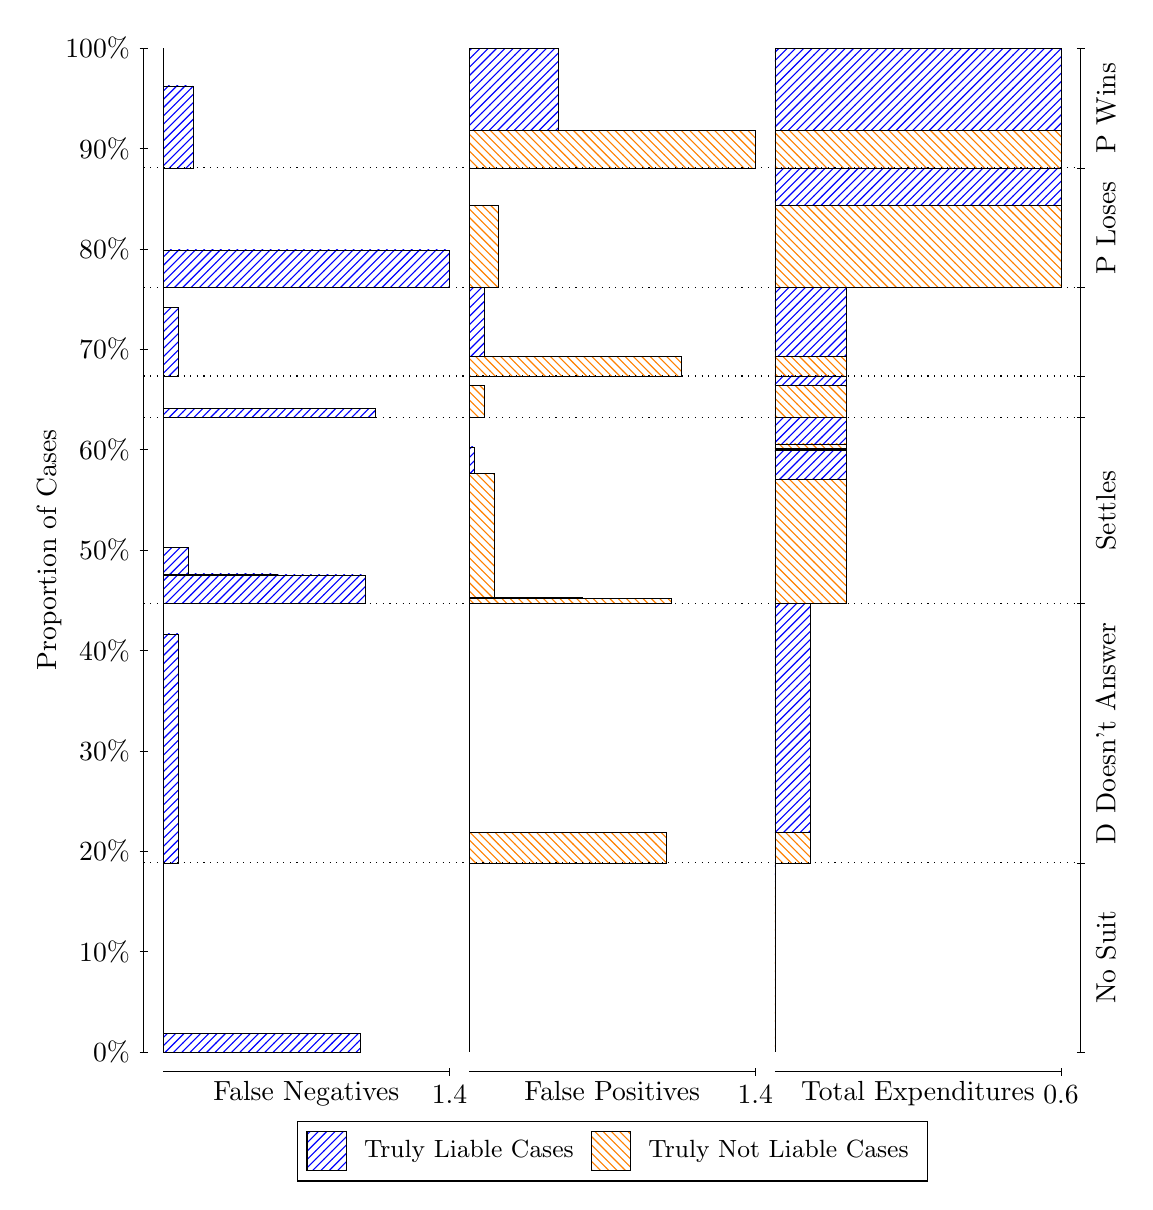
\begin{tikzpicture}
\draw[black, very thin] (1.5,1.75) -- (1.5,14.5);
\node[rotate=90, anchor=center] at (0.3, 8.125) {Proportion of Cases};
\draw[black, very thin] (1.45,1.75) -- (1.55,1.75);
\node[anchor=east] at (1.45, 1.75) {0\%};
\draw[black, very thin] (1.45,3.025) -- (1.55,3.025);
\node[anchor=east] at (1.45, 3.025) {10\%};
\draw[black, very thin] (1.45,4.3) -- (1.55,4.3);
\node[anchor=east] at (1.45, 4.3) {20\%};
\draw[black, very thin] (1.45,5.575) -- (1.55,5.575);
\node[anchor=east] at (1.45, 5.575) {30\%};
\draw[black, very thin] (1.45,6.85) -- (1.55,6.85);
\node[anchor=east] at (1.45, 6.85) {40\%};
\draw[black, very thin] (1.45,8.125) -- (1.55,8.125);
\node[anchor=east] at (1.45, 8.125) {50\%};
\draw[black, very thin] (1.45,9.4) -- (1.55,9.4);
\node[anchor=east] at (1.45, 9.4) {60\%};
\draw[black, very thin] (1.45,10.675) -- (1.55,10.675);
\node[anchor=east] at (1.45, 10.675) {70\%};
\draw[black, very thin] (1.45,11.95) -- (1.55,11.95);
\node[anchor=east] at (1.45, 11.95) {80\%};
\draw[black, very thin] (1.45,13.225) -- (1.55,13.225);
\node[anchor=east] at (1.45, 13.225) {90\%};
\draw[black, very thin] (1.45,14.5) -- (1.55,14.5);
\node[anchor=east] at (1.45, 14.5) {100\%};

\draw[black, very thin] (13.4,1.75) -- (13.4,14.5);
\draw[black, very thin] (13.35,1.75) -- (13.45,1.75);
\node[anchor=west] at (13.35, 1.75) {};
\draw[black, very thin] (13.35,4.1507) -- (13.45,4.1507);
\node[anchor=west] at (13.35, 4.1507) {};
\draw[black, very thin] (13.35,7.4478) -- (13.45,7.4478);
\node[anchor=west] at (13.35, 7.4478) {};
\draw[black, very thin] (13.35,9.8064) -- (13.45,9.8064);
\node[anchor=west] at (13.35, 9.8064) {};
\draw[black, very thin] (13.35,10.335) -- (13.45,10.335);
\node[anchor=west] at (13.35, 10.335) {};
\draw[black, very thin] (13.35,11.456) -- (13.45,11.456);
\node[anchor=west] at (13.35, 11.456) {};
\draw[black, very thin] (13.35,12.978) -- (13.45,12.978);
\node[anchor=west] at (13.35, 12.978) {};
\draw[black, very thin] (13.35,14.5) -- (13.45,14.5);
\node[anchor=west] at (13.35, 14.5) {};

\draw[black, very thin, pattern color=blue, pattern=north east lines] (1.75,1.75) rectangle (4.2557,1.991);
\draw[black, very thin, pattern color=orange, pattern=north west lines] (1.75,1.991) rectangle (1.75,4.1507);
\draw[black, very thin, pattern color=blue, pattern=north east lines] (1.75,4.1507) rectangle (1.9379,7.0609);
\draw[black, very thin, pattern color=orange, pattern=north west lines] (1.75,7.0609) rectangle (1.75,7.4478);
\draw[black, very thin, pattern color=blue, pattern=north east lines] (1.75,7.4478) rectangle (4.3184,7.8078);
\draw[black, very thin, pattern color=blue, pattern=north east lines] (1.75,7.8078) rectangle (3.1908,7.8205);
\draw[black, very thin, pattern color=blue, pattern=north east lines] (1.75,7.8205) rectangle (2.0632,8.1555);
\draw[black, very thin, pattern color=orange, pattern=north west lines] (1.75,8.1555) rectangle (1.75,9.8064);
\draw[black, very thin, pattern color=blue, pattern=north east lines] (1.75,9.8064) rectangle (4.4437,9.9262);
\draw[black, very thin, pattern color=orange, pattern=north west lines] (1.75,9.9262) rectangle (1.75,10.335);
\draw[black, very thin, pattern color=blue, pattern=north east lines] (1.75,10.335) rectangle (1.9379,11.209);
\draw[black, very thin, pattern color=orange, pattern=north west lines] (1.75,11.209) rectangle (1.75,11.456);
\draw[black, very thin, pattern color=blue, pattern=north east lines] (1.75,11.456) rectangle (5.3833,11.935);
\draw[black, very thin, pattern color=orange, pattern=north west lines] (1.75,11.935) rectangle (1.75,12.978);
\draw[black, very thin, pattern color=blue, pattern=north east lines] (1.75,12.978) rectangle (2.1259,14.02);
\draw[black, very thin, pattern color=orange, pattern=north west lines] (1.75,14.02) rectangle (1.75,14.5);
\draw[black, very thin, pattern color=orange, pattern=north west lines] (5.6333,1.75) rectangle (5.6333,3.9097);
\draw[black, very thin, pattern color=blue, pattern=north east lines] (5.6333,3.9097) rectangle (5.6333,4.1507);
\draw[black, very thin, pattern color=orange, pattern=north west lines] (5.6333,4.1507) rectangle (8.1391,4.5376);
\draw[black, very thin, pattern color=blue, pattern=north east lines] (5.6333,4.5376) rectangle (5.6333,7.4478);
\draw[black, very thin, pattern color=orange, pattern=north west lines] (5.6333,7.4478) rectangle (8.2017,7.5081);
\draw[black, very thin, pattern color=orange, pattern=north west lines] (5.6333,7.5081) rectangle (7.0741,7.5186);
\draw[black, very thin, pattern color=orange, pattern=north west lines] (5.6333,7.5186) rectangle (5.9466,9.0987);
\draw[black, very thin, pattern color=blue, pattern=north east lines] (5.6333,9.0987) rectangle (5.696,9.4337);
\draw[black, very thin, pattern color=blue, pattern=north east lines] (5.6333,9.4337) rectangle (5.6333,9.8064);
\draw[black, very thin, pattern color=orange, pattern=north west lines] (5.6333,9.8064) rectangle (5.8213,10.216);
\draw[black, very thin, pattern color=blue, pattern=north east lines] (5.6333,10.216) rectangle (5.6333,10.335);
\draw[black, very thin, pattern color=orange, pattern=north west lines] (5.6333,10.335) rectangle (8.327,10.582);
\draw[black, very thin, pattern color=blue, pattern=north east lines] (5.6333,10.582) rectangle (5.8213,11.456);
\draw[black, very thin, pattern color=orange, pattern=north west lines] (5.6333,11.456) rectangle (6.0092,12.498);
\draw[black, very thin, pattern color=blue, pattern=north east lines] (5.6333,12.498) rectangle (5.6333,12.978);
\draw[black, very thin, pattern color=orange, pattern=north west lines] (5.6333,12.978) rectangle (9.2667,13.457);
\draw[black, very thin, pattern color=blue, pattern=north east lines] (5.6333,13.457) rectangle (6.7609,14.5);
\draw[black, very thin, pattern color=orange, pattern=north west lines] (9.5167,1.75) rectangle (9.5167,3.9097);
\draw[black, very thin, pattern color=blue, pattern=north east lines] (9.5167,3.9097) rectangle (9.5167,4.1507);
\draw[black, very thin, pattern color=orange, pattern=north west lines] (9.5167,4.1507) rectangle (9.9708,4.5376);
\draw[black, very thin, pattern color=blue, pattern=north east lines] (9.5167,4.5376) rectangle (9.9708,7.4478);
\draw[black, very thin, pattern color=orange, pattern=north west lines] (9.5167,7.4478) rectangle (10.425,9.028);
\draw[black, very thin, pattern color=blue, pattern=north east lines] (9.5167,9.028) rectangle (10.425,9.3879);
\draw[black, very thin, pattern color=orange, pattern=north west lines] (9.5167,9.3879) rectangle (10.425,9.3984);
\draw[black, very thin, pattern color=blue, pattern=north east lines] (9.5167,9.3984) rectangle (10.425,9.4112);
\draw[black, very thin, pattern color=orange, pattern=north west lines] (9.5167,9.4112) rectangle (10.425,9.4714);
\draw[black, very thin, pattern color=blue, pattern=north east lines] (9.5167,9.4714) rectangle (10.425,9.8064);
\draw[black, very thin, pattern color=orange, pattern=north west lines] (9.5167,9.8064) rectangle (10.425,10.216);
\draw[black, very thin, pattern color=blue, pattern=north east lines] (9.5167,10.216) rectangle (10.425,10.335);
\draw[black, very thin, pattern color=orange, pattern=north west lines] (9.5167,10.335) rectangle (10.425,10.582);
\draw[black, very thin, pattern color=blue, pattern=north east lines] (9.5167,10.582) rectangle (10.425,11.456);
\draw[black, very thin, pattern color=orange, pattern=north west lines] (9.5167,11.456) rectangle (13.15,12.498);
\draw[black, very thin, pattern color=blue, pattern=north east lines] (9.5167,12.498) rectangle (13.15,12.978);
\draw[black, very thin, pattern color=orange, pattern=north west lines] (9.5167,12.978) rectangle (13.15,13.457);
\draw[black, very thin, pattern color=blue, pattern=north east lines] (9.5167,13.457) rectangle (13.15,14.5);
\draw[black, dotted] (1.5,4.1507) -- (13.4,4.1507);
\draw[black, dotted] (1.5,7.4478) -- (13.4,7.4478);
\draw[black, dotted] (1.5,9.8064) -- (13.4,9.8064);
\draw[black, dotted] (1.5,10.335) -- (13.4,10.335);
\draw[black, dotted] (1.5,11.456) -- (13.4,11.456);
\draw[black, dotted] (1.5,12.978) -- (13.4,12.978);
\draw[black, very thin] (1.75,1.5) -- (5.3833,1.5);
\node[anchor=north] at (3.5667, 1.5) {False Negatives};
\draw[black, very thin] (5.3833,1.45) -- (5.3833,1.55);
\node[anchor=north] at (5.3833, 1.45) {1.4};

\draw[black, very thin] (5.6333,1.5) -- (9.2667,1.5);
\node[anchor=north] at (7.45, 1.5) {False Positives};
\draw[black, very thin] (9.2667,1.45) -- (9.2667,1.55);
\node[anchor=north] at (9.2667, 1.45) {1.4};

\draw[black, very thin] (9.5167,1.5) -- (13.15,1.5);
\node[anchor=north] at (11.333, 1.5) {Total Expenditures};
\draw[black, very thin] (13.15,1.45) -- (13.15,1.55);
\node[anchor=north] at (13.15, 1.45) {0.6};

\node[black, centered, rotate=90] at (13.72, 2.9503) {No Suit};
\node[black, centered, rotate=90] at (13.72, 5.7993) {D Doesn't Answer};
\node[black, centered, rotate=90] at (13.72, 8.6271) {Settles};


\node[black, centered, rotate=90] at (13.72, 12.217) {P Loses};
\node[black, centered, rotate=90] at (13.72, 13.739) {P Wins};

\draw (7.449999999999999,1.5) node[draw=none] (baseCoordinate) {};
\begin{scope}[align=center]
        \matrix[scale=0.5, draw=black, below=0.5cm of baseCoordinate, nodes={draw}, column sep=0.1cm]{
            \node[rectangle, draw, minimum width=0.5cm, minimum height=0.5cm, pattern=north east lines, pattern color=blue] {}; &
            \node[draw=none, font=\small] (B) {Truly Liable Cases}; &
            \node[rectangle, draw, minimum width=0.5cm, minimum height=0.5cm, pattern=north west lines, pattern color=orange] {}; &
            \node[draw=none, font=\small] (B) {Truly Not Liable Cases}; \\
            };
\end{scope}

\end{tikzpicture}
\end{document}